% !Tex program = pdflatex
% 第 15 章: 辐射场与原子系统的相干相互作用
\ifx\allfiles\undefined
\documentclass{note}
\begin{document}
\fi
\setcounter{chapter}{18}
\chapter{光学电介质波导中的传播、调制和振荡}
\begin{exe}
    推导方程式 (19.2-7).
\end{exe}
\begin{pf}
    将课本式 (19.2-3)
    \begin{align}
        \mathcal{E}_y=\left\{\begin{array}{ll}
            C\exp(-qx),&0\leq x<\infty\\
            C[\cos(hx)-(q/h)\sin(hx)],&-t\leq x\leq 0,\\
            C[\cos(ht)+(q/h)\sin(ht)]\exp[p(x+t)],&-\infty<x\leq-t
        \end{array}\right.
    \end{align}
    代入式 (19.2-6)
    \begin{align}
        -\frac{1}{2}\int_{-\infty}^{\infty}E_yH_x^*\,\mathrm{d}x=\frac{\beta_m}{2\omega\mu}\int_{-\infty}^{\infty}[\mathcal{E}_y^{(m)}(x)]^2\,\mathrm{d}x=1
    \end{align}
    中得
    \begin{align}
        \notag&\frac{\beta_m}{2\omega\mu}\int_{-\infty}^{\infty}[\mathcal{E}_y^{(m)}(x)]^2\,\mathrm{d}x\\
        \notag=&C_m^2\frac{\beta_m}{2\omega\mu}\left\{\int_{-\infty}^{-t}\{[\cos(h_mt)+(q_m/h_m)\sin(h_mt)]\exp[p_m(x+t)]\}^2\,\mathrm{d}x+\int_{-t}^0[\cos(h_mx)-(q_m/h_m)\sin(h_mx)]^2\,\mathrm{d}x\right.\\
        \notag&\left.+\int_0^{\infty}[\exp(-q_mx)]^2\,\mathrm{d}x\right\}\\
        \notag=&C_m^2\frac{\beta_m}{2\omega\mu}\frac{1}{2h_m^2}\left(t+\frac{1}{q_m}+\frac{1}{p_m}\right)(h_m^2+q_m^2)=1,
    \end{align}
    故
    \begin{align}
        C_m=2h_m\left[\frac{\omega\mu}{\abs{\beta_m}\left(t+\frac{1}{q_m}+\frac{1}{p_m}\right)(h_m^2+q_m^2)}\right]^{1/2},
    \end{align}
    此即课本式 (19.2-7).
\end{pf}

\begin{exe}
    证明公式 (19.7-10) 的形式与模式功率守恒一致.
\end{exe}
\begin{pf}
    总模式功率
    \begin{align}
        P\propto\abs{A_m}^2+\abs{B_m}^2=A_m^*A_m+B_m^*B_m.
    \end{align}
    由课本式 (19.7-10)
    \begin{align}
        \frac{\mathrm{d}A_m}{\mathrm{d}z}=&-i\varkappa B_me^{-i(\beta_m^{\text{TM}}-\beta_m^{\text{TE}})z},\\
        \frac{\mathrm{d}B_m}{\mathrm{d}z}=&-i\varkappa A_me^{i(\beta_m^{\text{TM}}-\beta_m^{\text{TE}})z}.
    \end{align}
    故
    \begin{align}
        \notag\frac{\mathrm{d}P}{\mathrm{d}z}\propto&\frac{\mathrm{d}A_m^*}{\mathrm{d}z}A_m+A_m^*\frac{\mathrm{d}A_m}{\mathrm{d}z}+\frac{\mathrm{d}B_m^*}{\mathrm{d}z}B_m+B_m^*\frac{\mathrm{d}B_m}{\mathrm{d}z}\\
        \notag=&i\varkappa B_m^*e^{i(\beta_m^{\text{TM}}-\beta_m^{\text{TE}})z}A_m+A_m^*\left[-i\varkappa B_me^{-i(\beta_m^{\text{TM}}-\beta_m^{\text{TE}})z}\right]+i\varkappa A_m^*e^{-i(\beta_m^{\text{TM}}-\beta_m^{\text{TE}})z}B_m+B_m^*\left[-i\varkappa A_me^{i(\beta_m^{\text{TM}}-\beta_m^{\text{TE}})z}\right]\\
        =&0,h
    \end{align}
    即模式总功率守恒.
\end{pf}

\begin{exe}
    推导式 (19.7-12) 中的两个方程.
\end{exe}
\begin{pf}
    由课本式 (19.7-10)
    \begin{align}
        \label{19.3-1}
        \frac{\mathrm{d}A_m}{\mathrm{d}z}=&-i\varkappa B_me^{-i(\beta_m^{\text{TM}}-\beta_m^{\text{TE}})z},\\
        \label{19.3-2}
        \frac{\mathrm{d}B_m}{\mathrm{d}z}=&-i\varkappa A_me^{i(\beta_m^{\text{TM}}-\beta_m^{\text{TE}})z},
    \end{align}
    出发, 取式 \eqref{19.3-1} 关于 $z$ 的微分并利用式 \eqref{19.3-1} 和式 \eqref{19.3-2} 消去 $B_m$ 和 $\frac{\mathrm{d}B_m}{\mathrm{d}z}$ 得
    \begin{align}
        \frac{\mathrm{d}^2A_m}{\mathrm{d}z^2}+i(\beta_m^{\text{TM}}-\beta_m^{\text{TE}})\frac{\mathrm{d}A_m}{\mathrm{d}z}+\varkappa^2A_m=0,
    \end{align}
    考虑到边界条件 $A_m(0)=0$ 和 $\frac{\mathrm{d}A_m}{\mathrm{d}z}(0)=-i\varkappa B_0$, 解得
    \begin{align}
        A_m(z)=-iB_0e^{-i\delta z}\frac{\varkappa}{(\varkappa^2+\delta^2)^{1/2}}\sin[(\varkappa^2+\delta^2)^{1/2}z],
    \end{align}
    其中 $2\delta\equiv\beta_m^{\text{TM}}-\beta_m^{\text{TE}}$.
    将上式代回式 \eqref{19.3-1} 中可得
    \begin{align}
        B_m(z)=\frac{i}{\varkappa}\frac{\mathrm{d}A_m}{\mathrm{d}z}e^{i(\beta_m^{\text{TM}}-\beta_m^{\text{TE}})z}=B_0e^{i\delta z}\left\{\cos[(\varkappa^2+\delta^2)^{1/2}z]-i\frac{\delta}{(\kappa^2+\delta^2)^{1/2}}\sin[(\kappa^2+\delta^2)^{1/2}z]\right\},
    \end{align}
    此即课本式 (19.7-12).
\end{pf}

\begin{exe}
    考虑 19.8 节中讨论的能够将 TE 模转换到 TM 模, 磁光波导调制器的设计问题. 在模式的失配参量 $\delta$ 很大 (即 $\delta\gg\varkappa$) 的情况下, 需要考虑位相匹配的几种方法. 参照式 (19.8-16), 式 (19.8-17) 和式 (19.8-18), 是否能利用磁场 $H_z$ 的周期 (在 $z$ 方向) 性调制达到位相匹配? 需要的周期是多少? 将结果与参考文献 [20] 描述的解法进行比较.
\end{exe}
\begin{sol}
\end{sol}

\begin{exe}
    横向电光波调制器长度为 $L$ 和横截面为 $2\lambda\times 2\lambda$ ($\lambda$ 为真空中光的波长), 推导该调制器的调制功率表达式. 与体调制器的结果 (参考文献 [9], 第 325 页) 进行比较. 估算铌酸锂 (\ce{LiNbO_3}) 调制器在 $\lambda=1$ 微米, $L=5$ 毫米时所需要的功率.
\end{exe}
\begin{sol}
\end{sol}

\begin{exe}
    存在增益扰动的情况下, 即 $\gamma_1\neq 0$, $n_1=0$ 的情况下, 推导分布反馈激光器的振荡条件. 与参考文献 [17] 的结果进行比较.
\end{exe}
\begin{sol}
    存在增益扰动 (即 $\gamma_1\neq 0$, $n_1=0$) 的情况下,
    \begin{align}
        \varkappa=&i\frac{\gamma}{2},\\
        S^2=&\varkappa^2+(\gamma-i\Delta\beta)^2=-\frac{\gamma^2}{4}+(\gamma-i\Delta\beta)^2.
    \end{align}
    振荡条件为
    \begin{align}
        \frac{S-(\gamma-i\Delta\beta)}{S+(\gamma-i\Delta\beta)}e^{2SL}=-1.
    \end{align}
\end{sol}

\begin{exe}
    在 $n_1=1$, $n_2=3.5$, $n_3=3.4$, $t=3$ 微米, $a=500$ 埃, $\lambda=0.85$ 微米, $L=100$, $300$, $500$ 微米的情况下, 计算无损耗的砷化镓 (\ce{GaAs}) 分布反馈激光器的阈值增益常数. 画出增益与 $L$ 的关系曲线.
\end{exe}
\begin{sol}
    假设方波纹状周期性波导的折射率改变量空间周期 $\Lambda=0.11\,\mu$m, 激光模式为基模, 且处于完全束缚状态 (模式频率远远超过传播截止值) 下.
    此时激光模式的传输常数 $\beta_s=\beta_1\approx\frac{2\pi n_2}{\lambda}$, 周期性波导的空间频率为 $\frac{2l\pi}{\Lambda}=\frac{2\pi}{\Lambda}$ 与之耦合, 从而满足相位匹配条件
    \begin{align}
        \frac{2l\pi}{\Lambda}-\beta_s\approx\beta_s,
    \end{align}
    此时相位适配因子 (的一半) 为
    \begin{align}
        \Delta\beta=\beta_s-\frac{l\pi}{\Lambda}=-2.688\times 10^6\,\text{m}^{-1}.
    \end{align}
    耦合常数为
    \begin{align}
        \varkappa\approx\frac{2\pi^2s^2}{3l\lambda}\frac{n_2^2-n_1^2}{n_2}\left(\frac{a}{t}\right)^3\left[1+\frac{3}{2\pi}\frac{\lambda/a}{(n_2^2-n_1^2)^{1/2}}+\frac{3}{4\pi^2}\frac{(\lambda/a)^2}{(n_2^2-n_1^2)}\right]=618.8\,\text{m}^{-1}.
    \end{align}
    由
    \begin{align}
        \frac{e^{2\gamma L}}{\gamma^2}=\frac{4}{\varkappa^2}
    \end{align}
    得阈值增益 $\gamma$ 与长度 $L$ 的关系曲线如图 \ref{19.7-fig} 所示, 在 $L=100$, $300$, $500\,\mu$m 的情况下, 阈值增益 $\gamma$ 分别为 $900$ cm$^{-1}$, $300$ cm$^{-1}$, $180$ cm$^{-1}$.
    \begin{figure}[H]
        \centering
        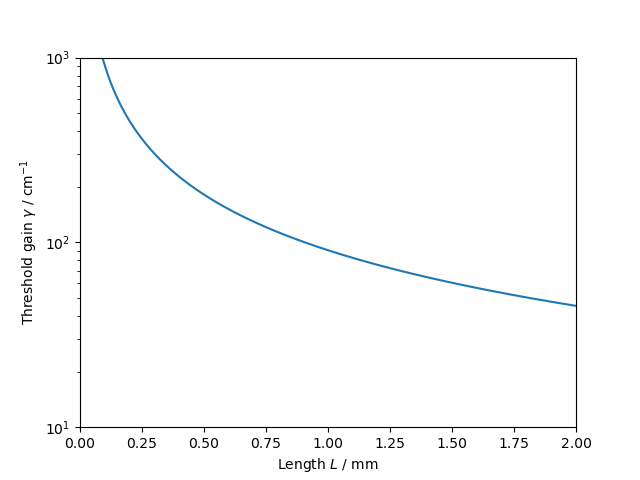
\includegraphics[width=.5\columnwidth]{Figures/19.7.png}
        \caption{阈值增益 $\gamma$ 与长度 $L$ 之间的关系曲线.}
        \label{19.7-fig}
    \end{figure}
\end{sol}

\begin{exe}
    对于如图 19.15 所示的漏泄型波导, 推导 TM 模的传播常数 $\gamma$.
\end{exe}
\begin{sol}
\end{sol}

\begin{exe}
    写出利用棱镜耦合器和光栅耦合器发射波导模的理论和实践的简短报告. 基础材料参见补充参考文献 [1] 和 [2].
\end{exe}
\begin{sol}
\end{sol}

\begin{exe}
    利用一维薛定谔方程和波动方程 (19.1-3) 之间形式上的相似性, 证明在无损耗波导中存在类似式 (1.2-5) 的方程\\
    在 $l\neq 0$ 时,
    \[
        \int_{-\infty}^{\infty}\mathcal{E}_y^{(l)}(x)\mathcal{E}_y^{(m)}(x)\,\mathrm{d}x=0
    \]
    提示: 为了在两个微分方程之间建立相似关系, 假定解具有式 (19.2-2) 的形式.
\end{exe}
\begin{pf}
    将课本中波动方程 (19.1-3)
    \begin{align}
        \left(\frac{\partial^2}{\partial x^2}+\frac{\partial^2}{\partial y^2}\right)\bm{E}(x,y)+[k^2n^2(\bm{r})-\beta^2]\bm{E}(x,y)=0
    \end{align}
    中的 $\bm{E}(x,y)$ 换成 $\mathcal{E}^{(l)}(x)$ 和 $\mathcal{E}_y^{(m)}(x)$ 得
    \begin{align}
        \label{19.10-1}
        \nabla^2\mathcal{E}_y^{(l)}(x)+[k^2n^2-(\beta^{(l)})^2]\mathcal{E}_y^{(l)}(x)=&0,\\
        \label{19.10-2}
        \nabla^2\mathcal{E}_y^{(m)}(x)+[k^2n^2-(\beta^{(m)})^2]\mathcal{E}_y^{(m)}(x)=&0.
    \end{align}
    将式 \eqref{19.10-1} 乘 $\mathcal{E}_y^{(m)}(x)$, 将式 \eqref{19.10-2} 乘 $\mathcal{E}_y^{(l)}(x)$, 再将两者相减得
    \begin{align}
        \mathcal{E}_y^{(m)}\nabla^2\mathcal{E}_y^{(l)}+\mathcal{E}_y^{(l)}\nabla^2\mathcal{E}_y^{(m)}=[(\beta^{(l)})^2-(\beta^{(m)})^2]\mathcal{E}_y^{(l)}\mathcal{E}_y^{(m)}.
    \end{align}
    上式关于全空间积分得
    \begin{align}
        \iiint_{\text{全空间}}[\mathcal{E}_y^{(m)}\nabla^2\mathcal{E}_y^{(l)}+\mathcal{E}_y^{(l)}\nabla^2\mathcal{E}_y^{(m)}]\,\mathrm{d}v=[(\beta^{(l)})^2-(\beta^{(m)})^2]\iiint_{\text{全空间}}\mathcal{E}_y^{(l)}\mathcal{E}_y^{(m)}\,\mathrm{d}v.
    \end{align}
    再利用格林定理得
    \begin{align}
        \iint_{\text{包围全空间的二维闭合曲面}}[\mathcal{E}_y^{(m)}\nabla\mathcal{E}_y^{(l)}+\mathcal{E}_y^{(l)}\nabla\mathcal{E}_y^{(m)}]\cdot\bm{n}\,\mathrm{d}a=[(\beta^{(l)})^2-(\beta^{(m)})^2]\iiint_{\text{全空间}}\mathcal{E}_y^{(l)}\mathcal{E}_y^{(m)}\,\mathrm{d}v.
    \end{align}
    由于无穷远处 $\mathcal{E}_y^{(l/m)}$ 和 $\mathcal{E}_y^{(l/m)}$ 均 $\rightarrow 0$, 故
    \begin{align}
        [(\beta^{(l)})^2-(\beta^{(m)})^2]\iiint_{\text{全空间}}\mathcal{E}_y^{(l)}\mathcal{E}_y^{(m)}\,\mathrm{d}v=0.
    \end{align}
    又因为对 $l\neq m$, 通常 $(\beta^{(l)})^2\neq(\beta^{(m)})^2$, 故
    \begin{gather}
        \iiint_{\text{全空间}}\mathcal{E}_y^{(l)}(x)\mathcal{E}_y^{(m)}(x)\,\mathrm{d}v=0,\\
        \Longrightarrow\int_{-\infty}^{\infty}\mathcal{E}_y^{(l)}(x)\mathcal{E}_y^{(m)}(x)\,\mathrm{d}x=0.
    \end{gather}
\end{pf}
\ifx\allfiles\undefined
\end{document}
\fi